% !TEX root =  ../main_manuscript.tex 
\section{Results}
The cause-specific cumulative upgrading-risk at year five of follow-up was 35\% in PRIAS and at most 50\% in validation cohorts (Panel~B, Figure~\ref{fig:auc_beforecalib}). Hence, many patients do not require all biopsies planned in the first five years of AS. In the fitted PRIAS model, the adjusted hazard ratio (aHR) of upgrading for an increase in patient age from 61 to 71 years (25-th to 75-th percentile) was 1.45~(95\%CI:~1.30--1.63). For an increase in fitted PSA value from 2.36 to 3.07 (25-th to 75-th percentile, log scale), the aHR was 0.99~(95\%CI:~0.89--1.11). The strongest predictor of upgrading-risk was instantaneous PSA velocity, with an increase from -0.09 to 0.31 (25-th to 75-th percentile), giving an aHR of 2.47~(95\%CI:~1.93--2.99). The aHR for PSA value and velocity varied between GAP3 cohorts (Supplementary~Table~8).

The time-dependent AUC, calibration plot, and time-dependent MAPE of our model are shown in Figure~\ref{fig:auc_beforecalib}, and Supplementary~Figure~8. In all cohorts, time-dependent AUC was moderate (0.55 to 0.75) over the whole follow-up period. Time-dependent MAPE was large (0.3 to 0.45) in those cohorts where the impact of PSA on upgrading-risk was different from PRIAS (e.g., MUSIC cohort, Supplementary~Table~8), and moderate (0.1 to 0.3) otherwise. In all cohorts, the MAPE decreased rapidly after year one of follow-up. Our model was miscalibrated for validation cohorts (Panel~B, Figure~\ref{fig:auc_beforecalib}). Recalibrating the baseline hazard of upgrading in validation cohorts resolved this issue (Supplementary~Figure~6). We compared risk predictions from the recalibrated models, with predictions from separately fitted cohort-specific joint models (Supplementary~Figure~7). The difference in predictions was lowest in Johns Hopkins cohort (impact of PSA on upgrading-risk similar to PRIAS). Comprehensive results are in Supplementary~A.2~and~B.

\begin{figure}
\centerline{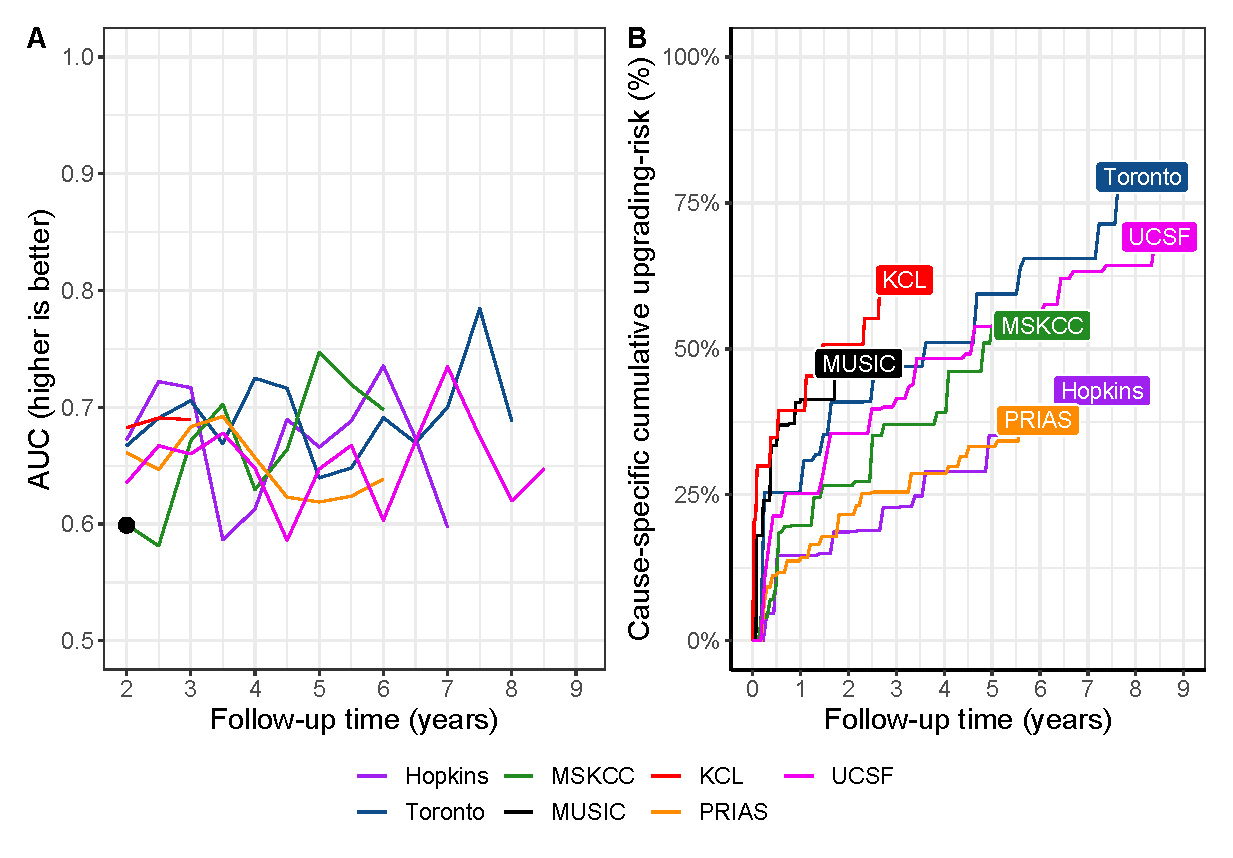
\includegraphics[width=\columnwidth]{images/auc_beforecalib.eps}}
\caption{\textbf{Model Validation Results}. \textbf{Panel~A}: time-dependent area under the receiver operating characteristic curve or AUC (measure of discrimination). \textbf{Panel~B}: calibration-at-large indicates model miscalibration. This is because solid lines depicting the non-parameteric estimate of the cause-specific cumulative upgrading-risk~\citep{turnbull1976empirical}, and dashed lines showing the average cause-specific cumulative upgrading-risk obtained using the joint model fitted to the PRIAS dataset, are not overlapping. Recalibrating the baseline hazard of upgrading resolved this issue (Supplementary~Figure~6). Full names of Cohorts are \textit{PRIAS}: Prostate Cancer International Active Surveillance, \textit{Toronto}: University of Toronto Active Surveillance, \textit{Hopkins}: Johns Hopkins Active Surveillance, \textit{MSKCC}: Memorial Sloan Kettering Cancer Center Active Surveillance, \textit{KCL}: King's College London Active Surveillance, \textit{MUSIC}: Michigan Urological Surgery Improvement Collaborative Active Surveillance, \textit{UCSF}: University of California San Francisco AS.}
\label{fig:auc_beforecalib}
\end{figure}

\subsection{Personalized Biopsy Schedules}
We employed the PRIAS based fitted model to create personalized biopsy schedules for real PRIAS patients. Specifically, first using the model and patient's observed data, we predicted his cumulative upgrading-risk (Figure~\ref{fig:demo_pat1}) on all of his future follow-up visits (biannually in PRIAS). Subsequently, we planned biopsies on those future visits where his conditional cumulative upgrading-risk was more than a certain threshold (Supplementary~Figure~9). Example personalized schedules based on 5\% and 10\% risk thresholds are shown in Figure~\ref{fig:demo_pat1}, and in Supplementary~Figure~10--12. For both personalized and fixed schedules, we estimated the expected time delay in detecting upgrading if the patient progresses before the time of the last planned biopsy (Panel~C, Figure~\ref{fig:demo_pat1}). This delay is also personalized (Supplementary~C.1). That is, even if two different patients are prescribed the same biopsy schedule, their expected delays will depend on their individual upgrading-risk profiles. Patients/doctors can utilize the expected delay and schedule of biopsies as criteria to compare fixed, and different risk-based personalized schedules.

\begin{figure}
\centerline{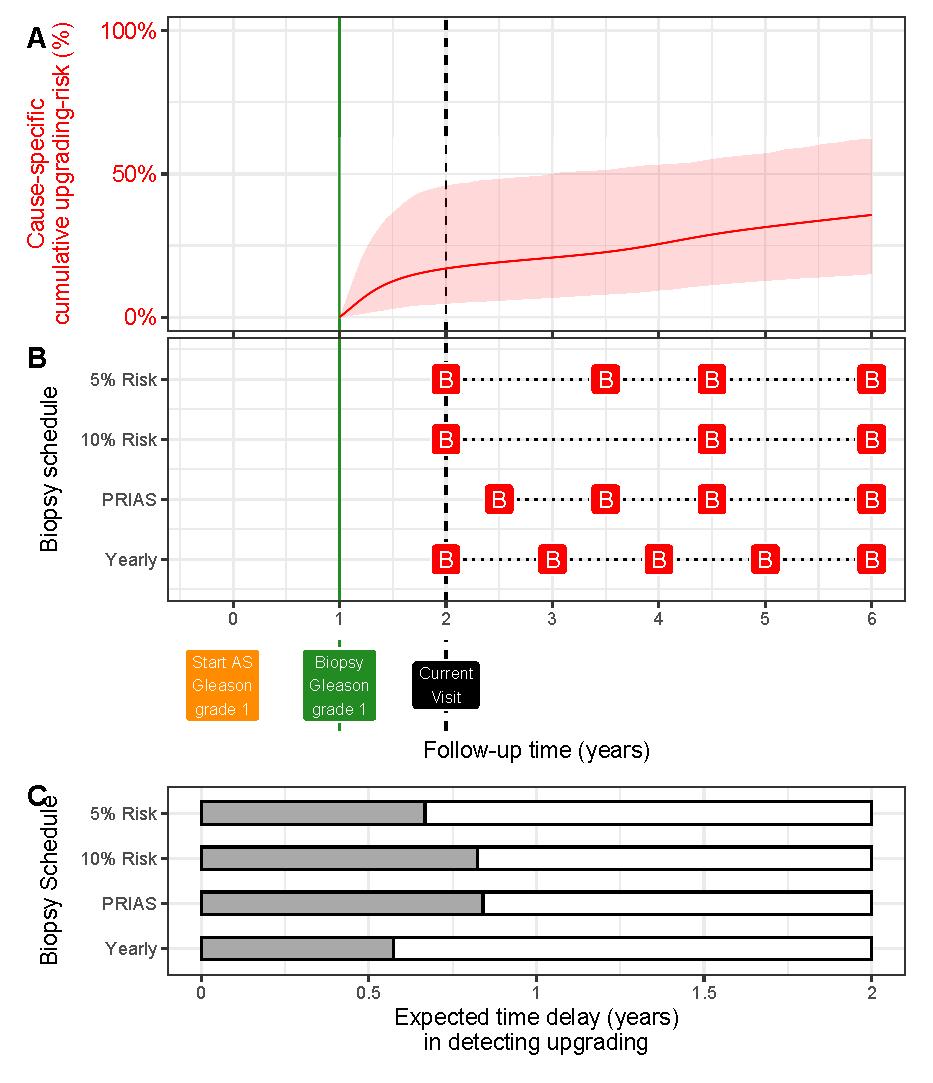
\includegraphics[width=\columnwidth]{images/demo_pat1.eps}}
\caption{\textbf{Illustration of personalized and fixed schedules of biopsies for patient from Figure~\ref{fig:jmExplanationPlot_113}}. \textbf{Panel~A:} Predicted cumulative upgrading-risk (95\% credible interval shaded). \textbf{Panel~B:} Different biopsy schedules with a red `B' indicating a future biopsy. Risk:~5\% and Risk:~10\% are personalized schedules in which a biopsy is planned whenever the conditional cause-specific cumulative upgrading-risk is above 5\% or 10\% risk, respectively. Green vertical line at year one is the time of the latest negative biopsy. Black dashed line at year two denotes the time of the current visit. \textbf{Panel~C:}\ Expected time delay in detecting upgrading (years) if patient progresses before year six. A compulsory biopsy was scheduled at year six (maximum biopsy scheduling time in PRIAS, Supplementary~C) in all schedules for a meaningful comparison between them.}
\label{fig:demo_pat1}
\end{figure}

\subsection{Web-Application}
We implemented our model and personalized schedules in a user-friendly web-application \url{https://emcbiostatistics.shinyapps.io/prias_biopsy_recommender/}. Currently, the web-application supports PRIAS and the six validation cohorts. Patient data can be entered manually and in Microsoft Excel format. Predictions for upgrading-risk are available for a currently limited, cohort-specific, follow-up period (Supplementary~Table~9). The web-application visualizes the timing of biopsies, and expected time delay in detecting upgrading, for personalized schedules based on 5\%, 10\%, and 15\% risk threshold; annual biopsies; biennial biopsies; and PRIAS schedule.